\documentclass{article}

%w | ! clear; pdflatex %
%https://tex.stackexchange.com/questions/20784/which-package-can-be-used-to-draw-automata
%https://www3.nd.edu/~dchiang/teaching/theory/2018/www/tikz_tutorial.pdf
\usepackage{tikz}
\usetikzlibrary{automata, positioning, arrows}

\begin{document}

Question 1a)

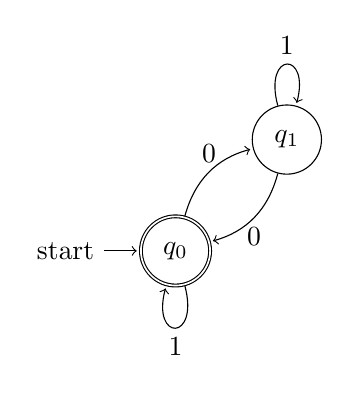
\begin{tikzpicture}[shorten >=1pt, node distance=2cm, on grid, auto]
    \node[state, initial, accepting] (q_0) {$q_0$};
    \node[state] (q_1) [above right=of q_0] {$q_1$};
        \path[->]
        (q_0)   edge [bend left, above] node {0} (q_1)
                edge [loop below] node {1} ()
        (q_1)   edge [bend left, below] node {0} (q_0)
                edge [loop above] node {1} ();  

\end{tikzpicture}

\vspace{2cm}

Question 1b)
\vspace{1cm}
\newline
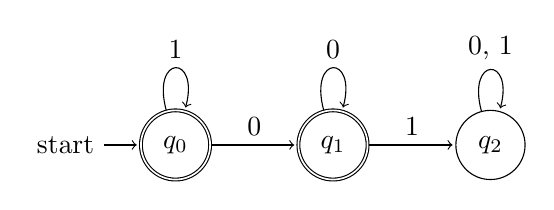
\begin{tikzpicture}[shorten >=1pt, node distance=2cm, on grid, auto]
    \node[state, initial, accepting] (q_0) {$q_0$};
    \node[state, accepting] (q_1) [right=of q_0] {$q_1$};
    \node[state] (q_2) [right=of q_1] {$q_2$};
        \path[->]
        (q_0)   edge node {0} (q_1)
                edge [loop above] node {1} ()
        (q_1)   edge node {1} (q_2)
                edge [loop above] node {0} ()
        (q_2)   edge [loop above] node {0, 1} ();

\end{tikzpicture}

\vspace{2cm}

Question 2a)
\vspace{1cm}
\newline

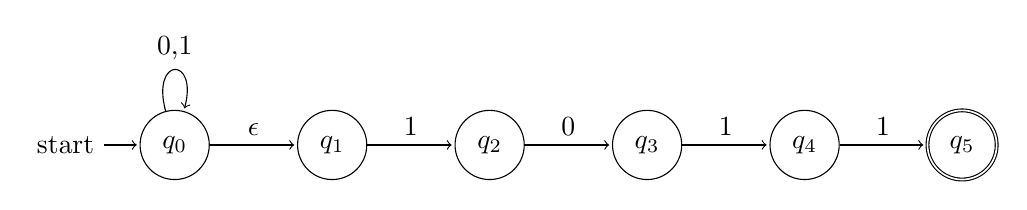
\begin{tikzpicture}[shorten >=1pt, node distance=2cm, on grid, auto]
    \node[state, initial] (q_0) {$q_0$};
    \node[state] (q_1) [right= of q_0] {$q_1$};
    \node[state] (q_2) [right= of q_1] {$q_2$};
    \node[state] (q_3) [right= of q_2] {$q_3$};
    \node[state] (q_4) [right= of q_3] {$q_4$};
    \node[state, accepting] (q_5) [right= of q_4] {$q_5$};
        \path[->]
        (q_0)   edge [loop above] node {0,1} ()
                edge node {$\epsilon$} (q_1)
        (q_1)   edge node {1} (q_2)
        (q_2)   edge node {0} (q_3)
        (q_3)   edge node {1} (q_4)
        (q_4)   edge node {1} (q_5);

\end{tikzpicture}

\end{document}

